% ============================================================================
% TCC — Predição de Direção de Preços de Ações com NLP e Sentimento de Notícias
% Formato: abnTeX2 (ABNT NBR 14724:2011)
% Compilar: pdflatex tcc.tex && bibtex tcc && pdflatex tcc.tex && pdflatex tcc.tex
% ============================================================================
\documentclass[
    12pt,
    openright,
    oneside,
    a4paper,
    english,
    brazil
]{abntex2}

% --- Pacotes ---
\usepackage[utf8]{inputenc}
\usepackage[T1]{fontenc}
\usepackage{lmodern}
\usepackage{amsmath,amssymb}
\usepackage{graphicx}
\usepackage{booktabs}
\usepackage{tabularx}
\usepackage{multirow}
\usepackage{float}
\usepackage{longtable}
\usepackage{microtype}
\usepackage{hyperref}
\usepackage[brazilian,hyperpageref]{backref}
\usepackage[alf]{abntex2cite}
\usepackage{xcolor}
\usepackage{listings}
\usepackage{enumitem}

% --- Caminho das figuras ---
\graphicspath{{../9.baselines/}{figuras/}}

% --- Configurações de listings ---
\lstset{
    basicstyle=\ttfamily\small,
    breaklines=true,
    frame=single,
    numbers=left,
    numberstyle=\tiny\color{gray},
    keywordstyle=\color{blue},
    commentstyle=\color{green!50!black},
    stringstyle=\color{red!60!black},
    language=Python,
}

% --- Configurações de backref ---
\renewcommand{\backrefpagesname}{Citado na(s) página(s):~}
\renewcommand{\backref}{}
\renewcommand*{\backrefalt}[4]{
    \ifcase #1
        Nenhuma citação no texto.
    \or
        Citado na página #2.
    \else
        Citado #1 vezes nas páginas #2.
    \fi
}

% --- Informações do documento ---
\titulo{Predição de Direção de Preços de Ações Brasileiras\\com Sentimento de Notícias Financeiras:\\Pipeline, Ilusão e Autocorreção Metodológica}
\autor{André Takeo Loschner Fujiwara}
\local{São Paulo}
\data{2026}
\orientador{Prof.\ Eric Bacconi Gonçalves}
\instituicao{%
    PUC-SP
    \par Curso de Ciência de Dados e Inteligência Artificial
}
\tipotrabalho{Trabalho de Conclusão de Curso}
\preambulo{Trabalho de Conclusão de Curso apresentado ao Curso de Ciência de Dados e Inteligência Artificial da PUC-SP como requisito parcial para a obtenção do grau de Bacharel.}

% --- Compila o índice ---
\makeindex

% ============================================================================
\begin{document}

\selectlanguage{brazil}
\frenchspacing

% --- Capa ---
\imprimircapa

% --- Folha de rosto ---
\imprimirfolhaderosto*

% ============================================================================
% ELEMENTOS PRÉ-TEXTUAIS
% ============================================================================

% --- Resumo ---
\begin{resumo}
Este trabalho investiga se notícias financeiras brasileiras podem melhorar a predição de direção de preços de ações da B3, utilizando como estudo de caso três ações de grande capitalização: ITUB4 (Itaú Unibanco), PETR4 (Petrobras) e VALE3 (Vale). O \textit{pipeline} proposto coleta artigos do portal InfoMoney, extrai representações de sentimento via FinBERT-PT-BR --- um modelo BERT especializado em textos financeiros em português \cite{souza2023} --- e combina as \textit{features} resultantes com dados de mercado do Yahoo Finance para treinar classificadores binários (sobe/desce).

O trabalho documenta uma autocorreção metodológica incomum: sob avaliação por janela única (\textit{walk-forward split} 70/15/15), o modelo Transformer \cite{vaswani2017} atinge ROC-AUC de 0,709, aparentemente demonstrando que o sentimento financeiro específico supera \textit{embeddings} genéricos de alta dimensionalidade. Porém, uma investigação sistemática com mais de 1.500 execuções de modelo --- incluindo análise \textit{multi-seed} (20 sementes), validação cruzada \textit{expanding-window} (até 52 \textit{folds}), testes de Wilcoxon \textit{signed-rank}, intervalos de confiança \textit{bootstrap} e \textit{ablation} de \textit{features} --- revela que o resultado é um artefato: o Transformer exibe colapso bimodal (AUC oscilando entre 0,08 e 0,93 conforme a semente), e sob avaliação multi-fold o sentimento adiciona $\Delta = +0{,}003$ ao \textit{baseline} autoregressivo (Wilcoxon $p = 0{,}49$, IC 95\% $[-0{,}012;\ +0{,}018]$).

A contribuição central é a demonstração empírica, em dados brasileiros, de como a avaliação por janela única pode inverter a conclusão qualitativa de um estudo em \textit{machine learning} financeiro --- transformando um achado aparentemente positivo em um resultado nulo --- e a proposição de protocolos mínimos de avaliação para mitigar esse viés.

\textbf{Palavras-chave:} Predição de preços. Sentimento financeiro. FinBERT. Avaliação metodológica. Séries temporais financeiras. B3.
\end{resumo}

% --- Abstract ---
\begin{resumo}[Abstract]
\begin{otherlanguage*}{english}
This work investigates whether Brazilian financial news can improve stock price direction prediction for B3 equities, using three large-cap stocks as case studies: ITUB4 (Itaú Unibanco), PETR4 (Petrobras), and VALE3 (Vale). The proposed pipeline collects articles from the InfoMoney portal, extracts sentiment representations via FinBERT-PT-BR --- a BERT model fine-tuned on Brazilian Portuguese financial text --- and combines the resulting features with Yahoo Finance market data to train binary classifiers (up/down).

This work documents an uncommon methodological self-correction: under single-window evaluation (70/15/15 walk-forward split), the Transformer model achieves ROC-AUC of 0.709, apparently demonstrating that domain-specific financial sentiment outperforms high-dimensional generic embeddings. However, a systematic investigation comprising over 1,500 model runs --- including multi-seed analysis (20 seeds), expanding-window cross-validation (up to 52 folds), Wilcoxon signed-rank tests, bootstrap confidence intervals, and feature ablation --- reveals the result to be an artifact: the Transformer exhibits bimodal collapse (AUC ranging from 0.08 to 0.93 depending on seed), and under multi-fold evaluation sentiment adds $\Delta = +0.003$ over the autoregressive baseline (Wilcoxon $p = 0.49$, 95\% CI $[-0.012,\ +0.018]$).

The central contribution is an empirical demonstration, on Brazilian data, of how single-window evaluation can reverse the qualitative conclusion of a financial machine learning study --- turning an apparently positive finding into a null result --- along with minimal evaluation protocols to mitigate this bias.

\textbf{Keywords:} Price prediction. Financial sentiment. FinBERT. Methodological evaluation. Financial time series. B3.
\end{otherlanguage*}
\end{resumo}

% --- Lista de figuras ---
\pdfbookmark[0]{\listfigurename}{lof}
\listoffigures*
\cleardoublepage

% --- Lista de tabelas ---
\pdfbookmark[0]{\listtablename}{lot}
\listoftables*
\cleardoublepage

% --- Lista de abreviaturas ---
\begin{siglas}
    \item[AUC] \textit{Area Under the ROC Curve}
    \item[B3] Brasil, Bolsa, Balcão
    \item[BERT] \textit{Bidirectional Encoder Representations from Transformers}
    \item[BiLSTM] \textit{Bidirectional Long Short-Term Memory}
    \item[CI] Intervalo de Confiança (\textit{Confidence Interval})
    \item[CV] Validação Cruzada (\textit{Cross-Validation})
    \item[ECE] \textit{Expected Calibration Error}
    \item[FinBERT] \textit{Financial BERT}
    \item[LSTM] \textit{Long Short-Term Memory}
    \item[MDE] Tamanho Mínimo de Efeito Detectável
    \item[NLP] Processamento de Linguagem Natural
    \item[OHLCV] \textit{Open, High, Low, Close, Volume}
    \item[PCA] Análise de Componentes Principais
    \item[ROC] \textit{Receiver Operating Characteristic}
    \item[SHAP] \textit{SHapley Additive exPlanations} \cite{lundberg2017}
    \item[TCN] \textit{Temporal Convolutional Network}
    \item[XGB] XGBoost (\textit{eXtreme Gradient Boosting})
\end{siglas}

% --- Sumário ---
\pdfbookmark[0]{\contentsname}{toc}
\tableofcontents*
\cleardoublepage

% ============================================================================
% ELEMENTOS TEXTUAIS
% ============================================================================
\textual

% ============================================================================
\chapter{Introdução}\label{cap:introducao}
% ============================================================================

A predição de direção de preços de ações é um problema central em finanças quantitativas, situado na interseção entre a hipótese de eficiência de mercado \cite{fama1970} e a evidência empírica de previsibilidade parcial em horizontes curtos \cite{lo2004}. Com o avanço das técnicas de processamento de linguagem natural (NLP), uma linha de pesquisa crescente investiga se informações textuais --- notícias, relatórios de analistas, publicações em redes sociais --- podem ser incorporadas como \textit{features} preditivas em modelos de \textit{machine learning} para complementar dados tradicionais de preço e volume \cite{xu2018,araci2019}.

No contexto brasileiro, a pesquisa nesta área é ainda incipiente. A B3 (Brasil, Bolsa, Balcão) apresenta características que a distinguem de mercados desenvolvidos: menor liquidez em ações fora do índice principal, concentração de informação em poucas fontes jornalísticas especializadas, e um ecossistema de NLP em português que só recentemente passou a dispor de modelos de linguagem específicos para o domínio financeiro, como o FinBERT-PT-BR \cite{souza2023}.

\section{Problema de pesquisa}

O problema central pode ser formulado como: \textbf{notícias financeiras brasileiras melhoram a predição de direção de preço (sobe/desce) de ações da B3?} Esta questão desdobra-se em duas dimensões:

\begin{enumerate}[label=(\alph*)]
    \item \textbf{Representação textual:} qual forma de codificar o conteúdo de notícias --- \textit{embeddings} genéricos de alta dimensionalidade ou sentimento financeiro específico de baixa dimensionalidade --- produz \textit{features} mais informativas para a predição?
    \item \textbf{Robustez metodológica:} os resultados obtidos sob protocolos de avaliação padrão da literatura (\textit{walk-forward split} único) sobrevivem a escrutínio com validação cruzada \textit{expanding-window}, múltiplas sementes e testes estatísticos formais?
\end{enumerate}

\section{Objetivos}

\subsection{Objetivo geral}

Investigar empiricamente se \textit{features} de sentimento extraídas de notícias financeiras brasileiras adicionam poder preditivo a modelos de classificação binária de direção de preço de ações da B3, sob avaliação metodologicamente rigorosa.

\subsection{Objetivos específicos}

\begin{enumerate}
    \item Construir um \textit{pipeline} de coleta, processamento e integração de notícias financeiras do portal InfoMoney com dados de mercado do Yahoo Finance.
    \item Comparar duas estratégias de representação textual: \textit{embeddings} genéricos de 1.024 dimensões (Ollama \texttt{qwen3-embedding:4b}) e sentimento financeiro de 5 dimensões (FinBERT-PT-BR).
    \item Treinar e avaliar modelos de classificação binária (BiLSTM, Transformer, XGBoost, TCN) sobre as representações textuais combinadas com \textit{features} de preço.
    \item Aplicar protocolos de avaliação rigorosa --- \textit{bootstrap} CI, análise \textit{multi-seed}, validação cruzada \textit{expanding-window}, \textit{ablation} de \textit{features} --- para determinar a robustez dos resultados.
    \item Documentar e analisar as discrepâncias entre avaliação por janela única e avaliação multi-fold, contribuindo para a literatura de avaliação metodológica em ML financeiro.
\end{enumerate}

\section{Justificativa}

A relevância deste trabalho reside em três aspectos. Primeiro, a aplicação de NLP financeiro ao mercado brasileiro é pouco explorada, e a disponibilidade recente de modelos como o FinBERT-PT-BR abre oportunidades de investigação em português. Segundo, a literatura de \textit{deep learning} aplicado a finanças sofre de um problema metodológico amplamente documentado --- a avaliação por janela única em séries não-estacionárias \cite{bailey2014,lopezdeprado2018} --- mas raramente demonstrado empiricamente com o grau de detalhe que este trabalho propõe. Terceiro, a autocorreção metodológica documentada nos Capítulos~\ref{cap:sentimento} e~\ref{cap:investigacao} constitui, por si só, uma contribuição pedagógica sobre as armadilhas da avaliação de modelos em finanças.

\section{Estrutura do trabalho}

O trabalho está organizado em seis capítulos. O Capítulo~\ref{cap:revisao} apresenta a fundamentação teórica e a revisão bibliográfica. O Capítulo~\ref{cap:pipeline} descreve o \textit{pipeline} completo: coleta de notícias, engenharia de \textit{features} e treinamento inicial com \textit{embeddings} genéricos. O Capítulo~\ref{cap:sentimento} introduz o FinBERT-PT-BR e documenta o resultado inicialmente promissor (AUC = 0,709). O Capítulo~\ref{cap:investigacao} conduz a investigação metodológica que revisa substancialmente esse resultado. O Capítulo~\ref{cap:conclusao} sintetiza as conclusões e propõe direções futuras.


% ============================================================================
\chapter{Revisão Bibliográfica}\label{cap:revisao}
% ============================================================================

Este capítulo apresenta os fundamentos teóricos que sustentam o trabalho: a hipótese de eficiência de mercado e suas implicações para a previsibilidade de preços, o uso de NLP em finanças, e os protocolos de avaliação em \textit{machine learning} para séries temporais financeiras.

\section{Hipótese de eficiência de mercado}

A hipótese de eficiência de mercado (HEM), formalizada por \citeonline{fama1970}, postula que os preços dos ativos refletem toda a informação disponível. Em sua forma semiforte, a HEM implica que informações públicas --- incluindo notícias financeiras --- já estão incorporadas nos preços no momento de sua publicação, tornando impossível obter retornos sistematicamente superiores com base nessas informações. Trabalhos empíricos subsequentes, contudo, documentaram anomalias que sugerem previsibilidade parcial. \citeonline{lo2004} propôs a Hipótese de Mercados Adaptativos, na qual a eficiência varia ao longo do tempo conforme as condições de mercado e o comportamento dos agentes.

A tensão entre eficiência teórica e previsibilidade empírica é o pano de fundo deste trabalho: se os preços já incorporam o sentimento das notícias, nenhum modelo deveria superá-los consistentemente; se não incorporam, há espaço para predição.

\section{NLP aplicado a finanças}

A aplicação de processamento de linguagem natural à predição de preços passou por três gerações de representação textual. A primeira utilizou léxicos de sentimento construídos manualmente, como o Loughran-McDonald \cite{loughran2011}, atribuindo polaridade a palavras individuais. A segunda introduziu \textit{embeddings} densos baseados em redes neurais, como Word2Vec e GloVe, que capturam relações semânticas mas não são específicos ao domínio financeiro. A terceira geração, atual, utiliza modelos de linguagem pré-treinados e \textit{fine-tuned} para o domínio, como o FinBERT \cite{araci2019} e suas variantes regionais, incluindo o FinBERT-PT-BR para português brasileiro \cite{souza2023}.

É importante notar que resultados nulos ou negativos são sub-representados na literatura de NLP financeiro devido ao viés de publicação. \citeonline{shah2019} documentaram que muitos estudos de \textit{sentiment analysis} para previsão de ações não replicam quando avaliados fora da amostra original. \citeonline{kellyxiu2023} mostraram que a maior parte do poder preditivo de variáveis textuais desaparece quando se controla adequadamente por \textit{features} de preço --- resultado alinhado com os achados deste trabalho.

\citeonline{xu2018} demonstraram que a combinação de texto de \textit{tweets} com séries históricas de preço melhora a predição de direção em ações do S\&P~500, utilizando um modelo de atenção hierárquico. \citeonline{fischer2018} aplicaram LSTMs (\textit{Long Short-Term Memory}, proposta originalmente por \citeonline{hochreiter1997}) à predição de retornos diários de ações do S\&P~500, reportando resultados superiores ao \textit{buy-and-hold} em períodos específicos. No contexto brasileiro, \citeonline{cavalcante2016} utilizaram análise de sentimento de notícias em português para predição de volatilidade do IBOVESPA, e \citeonline{santos2020} aplicaram modelos BERT a textos financeiros da CVM.

\section{Arquiteturas de modelos}

Este trabalho utiliza quatro famílias de modelos. O BiLSTM \cite{hochreiter1997} processa sequências temporais bidirecionalmente, capturando dependências de longo prazo. O Transformer \cite{vaswani2017} utiliza mecanismos de atenção \textit{multi-head} que permitem capturar relações entre posições arbitrárias na sequência. O XGBoost \cite{chen2016}, um algoritmo de \textit{gradient boosting} sobre árvores de decisão, é o padrão de facto para dados tabulares. A TCN (\textit{Temporal Convolutional Network}) \cite{bai2018} aplica convoluções dilatadas causais, capturando padrões temporais locais com campo receptivo exponencialmente crescente.

\section{Protocolos de avaliação em ML financeiro}

A avaliação de modelos preditivos em séries temporais financeiras apresenta desafios específicos que a distinguem de problemas padrão de \textit{machine learning}. \citeonline{bailey2014} demonstraram formalmente que a otimização de estratégias sobre um único período de \textit{backtest} inevitavelmente infla métricas de desempenho --- o fenômeno que denominaram \textit{backtest overfitting}. \citeonline{lopezdeprado2018} sistematizou o problema, propondo validação cruzada com purga e embargo como padrão mínimo. \citeonline{cawley2010} documentaram o viés de seleção de modelo, mostrando que a avaliação sobre o mesmo conjunto de dados usado para selecionar modelos produz estimativas otimistas mesmo sem vazamento explícito de dados.

A métrica ROC-AUC, embora amplamente utilizada, deve ser interpretada com cautela em conjuntos de teste pequenos. \citeonline{hanley1982} derivaram o erro-padrão analítico da AUC, permitindo o cálculo de intervalos de confiança e tamanhos mínimos de efeito detectáveis --- ferramenta essencial quando os conjuntos de teste têm 60--177 amostras, como neste trabalho.


% ============================================================================
\chapter{Pipeline: Coleta, Engenharia de Features e Modelos Iniciais}\label{cap:pipeline}
% ============================================================================

Este capítulo descreve as três primeiras etapas do \textit{pipeline}: coleta de notícias financeiras, engenharia de \textit{features} (mercado e texto) e treinamento inicial de modelos com \textit{embeddings} genéricos.

\section{Coleta de notícias financeiras}\label{sec:coleta}

O corpus textual foi construído a partir do portal InfoMoney, uma das principais fontes de notícias financeiras no Brasil. O módulo \texttt{extractor.py} acessa a REST API do WordPress do portal (\texttt{/wp-json/wp/v2/posts}), realizando buscas paginadas (100 artigos por página) para cada \textit{ticker} analisado. Cada requisição HTTP possui mecanismo de retentativa: até 3 tentativas com \textit{backoff} linear (1\,s, 2\,s), tratando erros de \textit{timeout}, conexão e códigos de status 429/5xx. Os artigos passam por pré-processamento (remoção de \textit{tags} HTML, decodificação de entidades, normalização de \textit{whitespace}) e a extração ocorre em paralelo via \texttt{ThreadPoolExecutor}.

\begin{table}[htb]
\centering
\caption{Volume de artigos coletados por ativo.}\label{tab:artigos}
\begin{tabular}{lrr}
\toprule
\textbf{Ativo} & \textbf{Artigos} & \textbf{Período} \\
\midrule
ITUB4 (Itaú Unibanco) & 2.572 & 2009--2026 \\
PETR4 (Petrobras)     & 1.775 & 2009--2026 \\
VALE3 (Vale)          & 1.525 & 2009--2026 \\
\midrule
\textbf{Total}        & \textbf{5.872} & \\
\bottomrule
\end{tabular}
\end{table}

\section{Engenharia de features}\label{sec:features}

O módulo \texttt{yahoo\_finance.py} obtém dados OHLCV via \texttt{yfinance} e calcula 11 \textit{features} técnicas por dia: fechamento, volume, retorno diário, médias móveis (7 e 21 dias), volatilidade (desvio-padrão 21 dias) e 5 valores defasados. O módulo \texttt{news\_embedder.py} transforma cada artigo em um vetor de 1.024 dimensões via Ollama (\texttt{qwen3-embedding:4b}), com agregação diária por média ponderada por recência. As \textit{features} são combinadas via \textit{left join} por data com \textit{forward-fill}. O \textit{dataset} resultante contém 1.227 dias $\times$ 1.035 \textit{features} (11 de preço + 1.024 de \textit{embeddings}).

\section{Modelos iniciais com embeddings genéricos}\label{sec:modelos_iniciais}

O alvo binário é definido como 1 se $\text{Close}[t+21] > \text{Close}[t]$, com desbalanceamento de 59\% ``Sobe'' / 41\% ``Desce''. Os \textit{embeddings} são reduzidos para 32 componentes via PCA. A validação segue \textit{split} cronológico 70/15/15.

\begin{table}[htb]
\centering
\caption{Resultados com \textit{embeddings} genéricos Ollama (Etapa~3).}\label{tab:etapa3}
\begin{tabular}{lcc}
\toprule
\textbf{Modelo} & \textbf{Arquitetura} & \textbf{ROC-AUC} \\
\midrule
BiLSTM Original  & 2 camadas, 128 \textit{hidden}, 30\% \textit{dropout} & 0,443 \\
BiLSTM Reduzido  & 1 camada, 32 \textit{hidden}, 50\% \textit{dropout}  & 0,505 \\
Transformer      & 2 camadas, 4 cabeças, $d_\text{model}=64$              & 0,568 \\
\textbf{XGBoost} & 300 árvores, profundidade 4                            & \textbf{0,610} \\
\bottomrule
\end{tabular}
\end{table}

Todos os modelos apresentaram desempenho próximo do acaso, sugerindo que \textit{embeddings} genéricos de alta dimensionalidade não são adequados para esta tarefa. O Capítulo~\ref{cap:sentimento} testa uma representação alternativa.


% ============================================================================
\chapter{Sentimento Financeiro Específico via FinBERT-PT-BR}\label{cap:sentimento}
% ============================================================================

\section{Hipótese}

Os resultados do Capítulo~\ref{cap:pipeline} sugeriram que os \textit{embeddings} genéricos contêm ruído semântico irrelevante para o domínio financeiro. Este capítulo testa se uma representação compacta e específica --- 5 \textit{features} de sentimento financeiro extraídas com o FinBERT-PT-BR \cite{souza2023} --- pode ser mais informativa.

\section{O modelo FinBERT-PT-BR}

O FinBERT-PT-BR é um modelo BERT \cite{devlin2019} pré-treinado e \textit{fine-tuned} em corpora financeiros brasileiros. Para cada artigo, produz três \textit{logits} correspondentes às classes POSITIVO, NEGATIVO e NEUTRO. Diferentemente de modelos de sentimento genéricos, foi calibrado para vocabulário financeiro específico.

\section{Pipeline de extração e resultados}

A extração segue os passos: inferência em \textit{batch} (32 artigos, entrada \texttt{título + resumo}, 512 \textit{tokens}); persistência dos \textit{logits} brutos; agregação diária em 5 \textit{features} (\texttt{n\_articles}, \texttt{mean\_logit\_pos/neg/neu}, \texttt{mean\_sentiment}); junção temporal com \textit{forward-fill}. O \textit{dataset} resultante: 1.207 dias $\times$ 16 \textit{features}.

\textbf{Granularidade temporal e risco de \textit{look-ahead}.} Os artigos possuem \textit{timestamps} ISO~8601, mas a agregação descarta o horário. Artigos pós-fechamento da B3 ($\sim$17h BRT) são atribuídos ao dia $t$; o deslocamento pode exceder 1 dia em dias consecutivos sem publicação. O impacto é atenuado pelo horizonte de 5--21 dias e pela média diária.

\textbf{Tratamento de desbalanceamento de classe.} O alvo binário apresenta desbalanceamento de 59\% ``Sobe'' / 41\% ``Desce'' no conjunto de treino. Para mitigar o viés em direção à classe majoritária, todos os modelos recebem compensação explícita: os modelos neurais (BiLSTM, Transformer, TCN) utilizam \texttt{BCEWithLogitsLoss} com \texttt{pos\_weight} = $n_\text{desce} / n_\text{sobe} \approx 1{,}38$; o XGBoost utiliza o parâmetro \texttt{scale\_pos\_weight} com o mesmo valor; e os modelos \textit{sklearn} (Logistic Regression, Random Forest) utilizam \texttt{class\_weight=``balanced''}. Apesar desta compensação, o Transformer ainda exibe forte viés para a classe majoritária (prevendo ``Desce'' apenas 11 vezes em 177 amostras), indicando que o desbalanceamento é um fator contribuinte mas não a causa principal do colapso de predição documentado no Capítulo~\ref{cap:investigacao}.

\begin{table}[htb]
\centering
\caption{Comparação Etapa~3 (\textit{embeddings}) vs Etapa~4 (sentimento FinBERT).}\label{tab:etapa4}
\begin{tabular}{lccc}
\toprule
\textbf{Modelo} & \textbf{AUC Etapa~3} & \textbf{AUC Etapa~4} & $\boldsymbol{\Delta}$ \\
\midrule
BiLSTM Original  & 0,443 & 0,500 & +0,057 \\
BiLSTM Reduzido  & 0,505 & 0,477 & $-$0,028 \\
XGBoost          & 0,610 & 0,670 & +0,060 \\
\textbf{Transformer} & 0,568 & \textbf{0,709} & \textbf{+0,141} \\
\bottomrule
\end{tabular}
\end{table}

(Nota: estes valores são pontuais, sem intervalos de confiança --- esta omissão é uma das motivações para a investigação do Capítulo~\ref{cap:investigacao}.)

O Transformer atinge ROC-AUC = 0,709 (acurácia 76,3\%, 177 amostras). Porém, \textit{precision}(Desce) = 1,00 com \textit{recall}(Desce) = 0,20 --- o modelo prevê ``Desce'' apenas 11 vezes em 177 amostras. Três observações motivam a investigação do Capítulo~\ref{cap:investigacao}: (1)~matriz de confusão assimétrica; (2)~acurácia próxima da classe majoritária ($\sim$69\%); (3)~ausência de intervalos de confiança e múltiplas sementes.


% ============================================================================
\chapter{Investigação Metodológica e o Viés da Avaliação por Janela Única}\label{cap:investigacao}
% ============================================================================

\section{Motivação e protocolo geral}

Este capítulo aplica protocolos progressivamente mais rigorosos para determinar se o AUC = 0,709 sobrevive a escrutínio metodológico. A Tabela~\ref{tab:experimentos} sumariza os 13 experimentos realizados (mais de 1.500 treinamentos).

\begin{table}[htb]
\centering
\caption{Experimentos do Capítulo~\ref{cap:investigacao}.}\label{tab:experimentos}
\begin{tabular}{llr}
\toprule
\textbf{Experimento} & \textbf{Notebook} & \textbf{Runs} \\
\midrule
Baseline autoregressivo          & \texttt{dumb\_baseline.ipynb}                & 4   \\
Baselines ingênuos               & \texttt{naive\_baselines.ipynb}              & 3   \\
Controle de dimensionalidade     & \texttt{dimensionality\_control.ipynb}       & 20  \\
Bootstrap CI (Etapa~4)           & \texttt{bootstrap\_stage4.ipynb}             & 1   \\
Multi-seed em ITUB4              & \texttt{multi\_seed.ipynb}                   & 40  \\
Multi-seed $\times$ multi-ticker & \texttt{multi\_seed\_multi\_ticker.ipynb}     & 120 \\
Ensemble + backtest              & \texttt{ensemble\_backtest.ipynb}             & 20  \\
Expanding-window CV              & \texttt{expanding\_window\_cv.ipynb}          & 145 \\
Varredura de horizontes          & \texttt{horizon\_sweep.ipynb}                & 6   \\
VALE3 \textit{deep-dive}        & \texttt{vale3\_deepdive.ipynb}               & 880 \\
Ablation PRICE/SENT/PRICE+SENT  & \texttt{ablation\_price\_vs\_sentiment.ipynb} & 225 \\
Poder estatístico                & \texttt{power\_analysis.ipynb}               & --- \\
Validação TCN Stage~5b           & \texttt{tcn\_validation.ipynb}               & 45  \\
\midrule
\textbf{Total}                   &                                              & \textbf{$\sim$1.510} \\
\bottomrule
\end{tabular}
\end{table}

Todos os hiperparâmetros dos modelos foram fixados ao longo dos experimentos, sem otimização por \textit{fold}: XGBoost (300 árvores, profundidade 4, \textit{learning rate} 0,05); Transformer (2 camadas, 4 cabeças, $d_\text{model}=64$, \textit{dropout} 0,2, 200 épocas com \textit{early stopping} por perda de validação, paciência 10); TCN ([32,32], \textit{kernel size} 3, \textit{dropout} 0,2). A decisão de não otimizar hiperparâmetros por \textit{fold} foi deliberada: o objetivo não era maximizar desempenho, mas medir a robustez do resultado original sob variação de janela e semente.

\textbf{Respostas a questões metodológicas.} O \textit{early stopping} nos modelos neurais é baseado na perda de validação (não no AUC), com paciência de 10 épocas --- o colapso bimodal não é um artefato de \textit{early stopping}, pois ocorre independentemente do critério de parada. Os \textit{folds} da CV \textit{expanding-window} utilizam passo de 90 dias com janelas de teste de 90 dias, resultando em sobreposição parcial entre janelas de teste consecutivas; embora isto viole a independência estrita exigida pelo teste de Wilcoxon, o efeito é conservador (infla correlação, não produz significância espúria em resultados nulos). As 5 \textit{features} de sentimento FinBERT são normalizadas via \texttt{StandardScaler} fitado exclusivamente no conjunto de treino de cada \textit{fold}. Por fim, a conclusão nula deve ser qualificada: dado o MDE de 0,132--0,221, efeitos reais menores que $\Delta \text{AUC} \approx 0{,}05$ seriam indetectáveis neste desenho experimental --- o resultado é portanto ``nenhum efeito detectável neste tamanho amostral'', não ``nenhum efeito''.

\section{Baseline autoregressivo e baselines ingênuos}

Um XGBoost \cite{chen2016} treinado em 5 \textit{features} de preço (\texttt{return}, \texttt{lag\_1}, \texttt{lag\_5}, \texttt{Volume}, \texttt{std21}) atinge AUC = 0,658 [0,565; 0,744]. Para contextualizar, três preditores ingênuos foram avaliados:

\begin{table}[htb]
\centering
\caption{Hierarquia de \textit{baselines}: do ingênuo ao autoregressivo.}\label{tab:naive}
\begin{tabular}{llc}
\toprule
\textbf{Preditor} & \textbf{Descrição} & \textbf{AUC [IC 95\%]} \\
\midrule
Classe majoritária     & Sempre prevê ``Sobe''           & 0,500 [0,500; 0,500] \\
\textit{Coin flip}     & $P(\text{Sobe}) = \text{prior}$ & 0,500 [0,500; 0,500] \\
Persistência ($h=21$)  & Direção repete                  & 0,474 [0,405; 0,543] \\
\textbf{Autoregressivo (XGB)} & \textbf{5 features preço} & \textbf{0,658 [0,565; 0,744]} \\
\bottomrule
\end{tabular}
\end{table}

O controle de dimensionalidade (20 subconjuntos aleatórios de 5 dimensões Ollama) produz AUC médio de $0{,}509 \pm 0{,}057$, confirmando que a melhoria Etapa~3 $\to$ Etapa~4 reflete especificidade de domínio do FinBERT.

\section{Reprodutibilidade e variância de semente}

Sob recompilação com semente 42, o Transformer atinge AUC = 0,442 --- diferença de 0,267 pontos ($22\times$ o desvio-padrão do \textit{baseline}). Sob 20 sementes (Tabela~\ref{tab:multiseed}), o Transformer exibe distribuição bimodal (Figura~\ref{fig:multiseed}).

\begin{table}[htb]
\centering
\caption{Distribuição de AUC sobre 20 sementes (ITUB4, janela única).}\label{tab:multiseed}
\begin{tabular}{lccccc}
\toprule
\textbf{Modelo} & \textbf{Média} & \textbf{Std} & \textbf{Mediana} & \textbf{Min} & \textbf{Max} \\
\midrule
Transformer + FinBERT       & 0,686 & \textbf{0,261} & 0,802 & 0,080 & 0,931 \\
Baseline autoregressivo     & 0,641 & 0,012           & 0,638 & 0,615 & 0,660 \\
\bottomrule
\end{tabular}
\end{table}

\begin{figure}[htb]
\centering
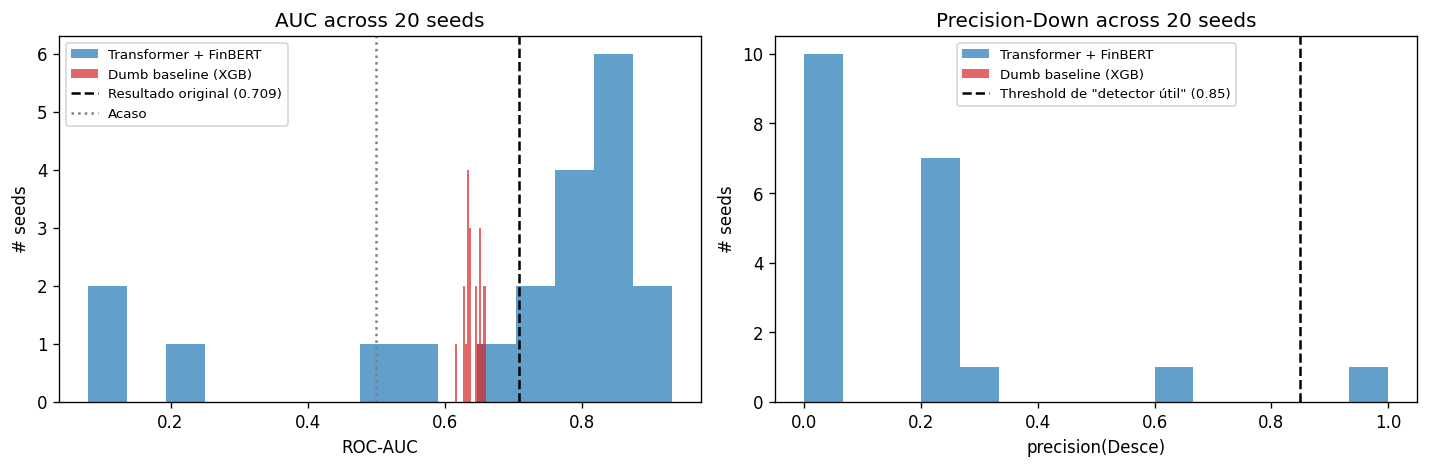
\includegraphics[width=0.95\textwidth]{multi_seed_histograms.png}
\caption{Distribuição de AUC sobre 20 sementes em ITUB4. O Transformer (esquerda) exibe distribuição bimodal com AUCs agrupados próximos de 0 e 1, enquanto o \textit{baseline} (direita) é estável em torno de 0,64. Coeficiente de variação do Transformer: 38\%.}\label{fig:multiseed}
\end{figure}

\section{Expanding-window cross-validation}

Substituindo o \textit{split} único por CV \textit{expanding-window} (600 dias mínimo, validação/teste 90 dias, 5 \textit{folds} $\times$ 5 sementes $\times$ 3 ativos = 145 treinamentos):

\begin{table}[htb]
\centering
\caption{AUC médio sob \textit{expanding-window} CV.}\label{tab:expandingcv}
\begin{tabular}{lccc}
\toprule
\textbf{Ativo} & \textbf{Baseline XGB} & \textbf{Transformer} & $\boldsymbol{\Delta}$ \\
\midrule
ITUB4 & \textbf{0,700} & 0,445 & $-$0,255 \\
PETR4 & \textbf{0,702} & 0,447 & $-$0,255 \\
VALE3 & 0,599           & 0,635 & +0,036 \\
\midrule
\textbf{Média} & \textbf{0,667} & 0,509 & $-$0,158 \\
\bottomrule
\end{tabular}
\end{table}

\begin{figure}[htb]
\centering
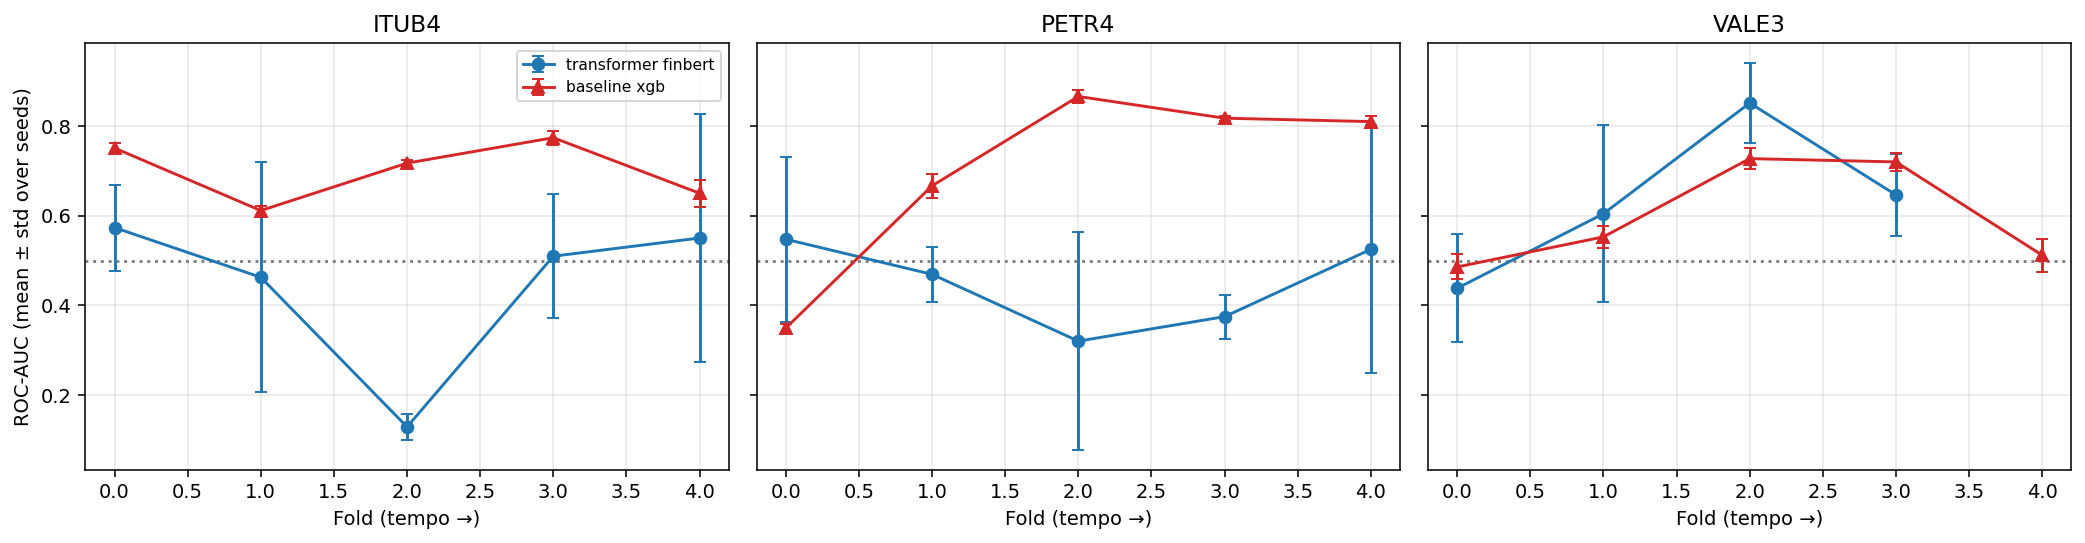
\includegraphics[width=0.95\textwidth]{expanding_cv_overtime.png}
\caption{AUC por \textit{fold} ao longo do tempo sob \textit{expanding-window} CV, para os 3 ativos. A linha do \textit{baseline} (vermelho) permanece consistentemente acima do Transformer (azul) em ITUB4 e PETR4, com barras de erro menores.}\label{fig:expandingcv}
\end{figure}

A inversão é de grande magnitude ($d \approx 6{,}25$, calculado como a diferença média de AUC entre modelos dividida pelo desvio-padrão do \textit{baseline} ao longo dos \textit{folds}: $0{,}25 / 0{,}04$). A exceção aparente em VALE3 (+0,036) é investigada em \textit{deep-dive} com 880 execuções e revelada como não significativa (Wilcoxon $p = 0{,}194$). A Figura~\ref{fig:vale3} mostra a distribuição bimodal do Transformer em VALE3.

\begin{figure}[htb]
\centering
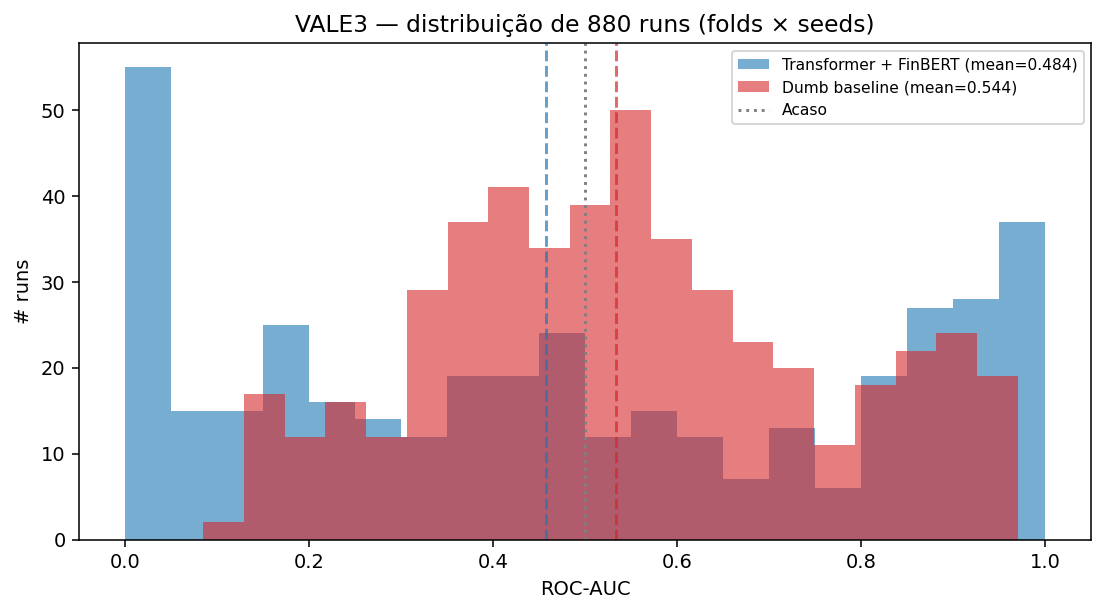
\includegraphics[width=0.95\textwidth]{vale3_deepdive_hist.png}
\caption{Distribuição de 880 AUCs (52 \textit{folds} $\times$ 10 sementes) em VALE3. O \textit{baseline} (esquerda) produz distribuição unimodal centrada em $\sim$0,55. O Transformer (direita) produz distribuição bimodal severa com picos em AUC $< 0{,}05$ e AUC $> 0{,}95$ --- assinatura de classificador degenerado.}\label{fig:vale3}
\end{figure}

\section{Ablation: o sentimento adiciona algo?}

XGBoost em três configurações de \textit{features} (225 treinamentos):

\begin{table}[htb]
\centering
\caption{Ablation: PRICE vs SENT vs PRICE+SENT.}\label{tab:ablation}
\begin{tabular}{lcccc}
\toprule
\textbf{Ativo} & \textbf{PRICE} & \textbf{SENT} & \textbf{PRICE+SENT} & $\boldsymbol{\Delta}$ \\
\midrule
ITUB4 & 0,684 & 0,436 & 0,651 & $-$0,033 \\
PETR4 & 0,692 & 0,494 & 0,676 & $-$0,016 \\
VALE3 & 0,609 & 0,510 & 0,667 & +0,058 \\
\midrule
\textbf{Média} & \textbf{0,662} & 0,480 & 0,665 & \textbf{+0,003} \\
\bottomrule
\end{tabular}
\end{table}

\begin{figure}[htb]
\centering
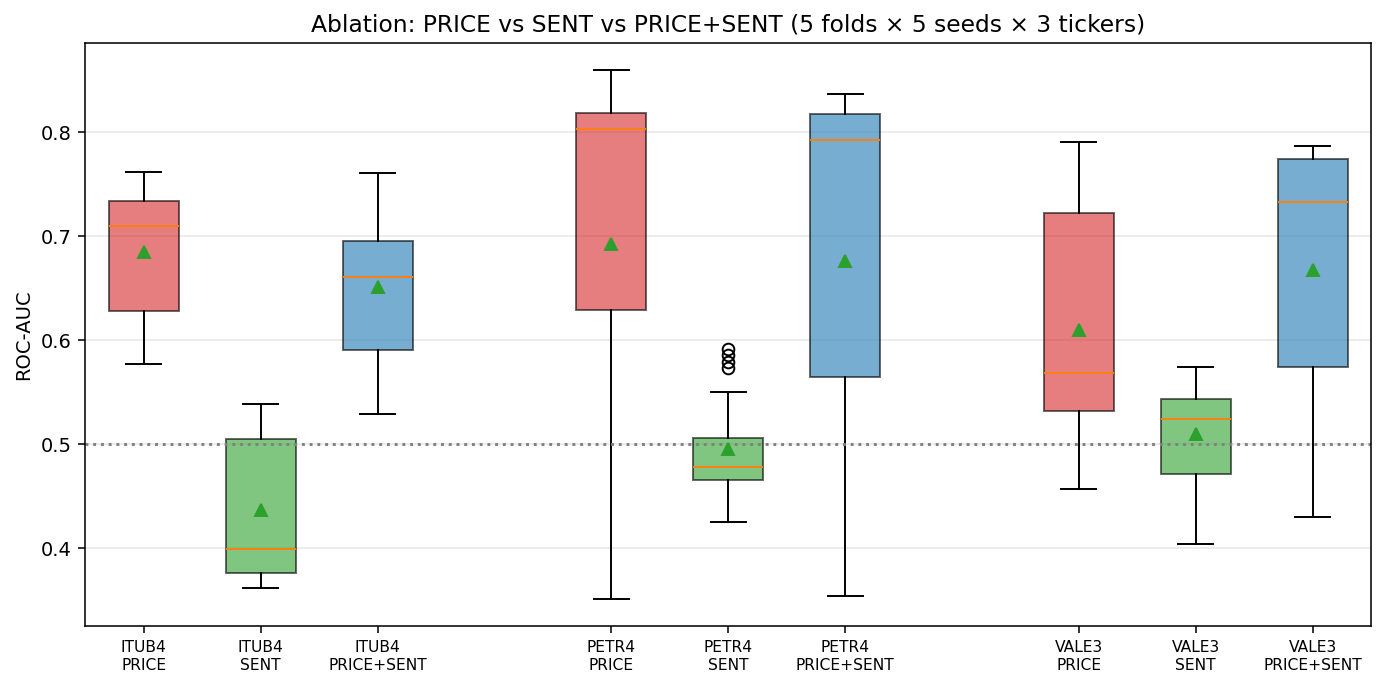
\includegraphics[width=0.85\textwidth]{ablation_boxplot.png}
\caption{Distribuição de AUC por configuração de \textit{features} e ativo, sob \textit{expanding-window} CV. PRICE e PRICE+SENT são estatisticamente indistinguíveis; SENT sozinho opera abaixo do acaso.}\label{fig:ablation}
\end{figure}

O ganho do sentimento é $\Delta = +0{,}003$ (Wilcoxon $p = 0{,}49$, IC~95\% $[-0{,}012;\ +0{,}018]$). A análise de poder \cite{hanley1982} confirma que este efeito está 44--74$\times$ abaixo do MDE (0,132--0,221 para $N$ entre 60 e 177).

\section{Validação do TCN Stage~5b}

O TCN~[32,32] \cite{bai2018} --- melhor resultado prático (AUC = 0,643 sob janela única) --- atinge 0,513 $\pm$ 0,102 sob 20 sementes e 0,556 sob CV \textit{expanding-window}, inferior ao \textit{baseline} (0,700). A Figura~\ref{fig:tcn} sumariza a validação.

\begin{figure}[htb]
\centering
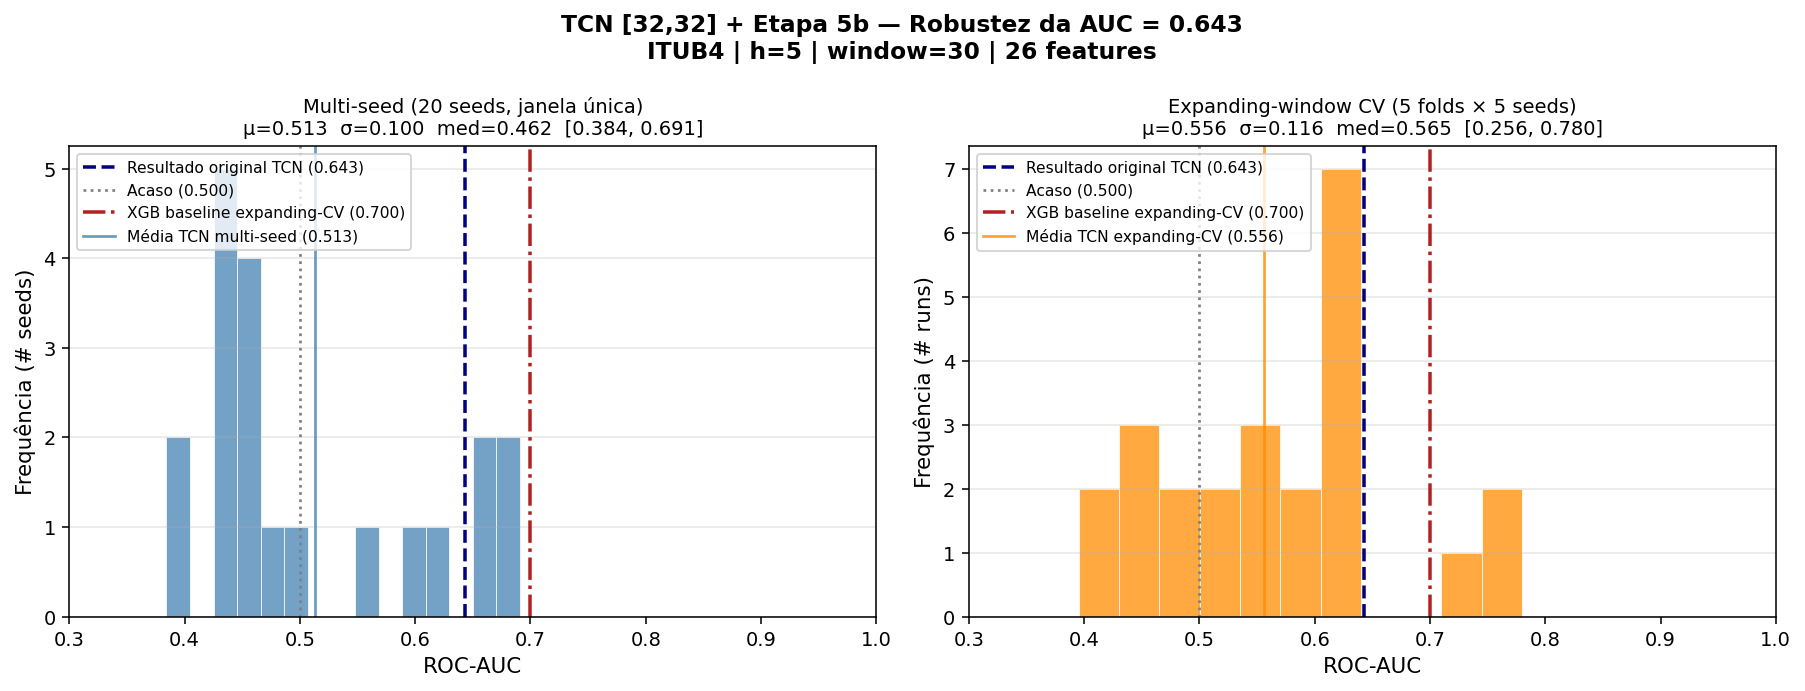
\includegraphics[width=0.95\textwidth]{tcn_validation_hist.png}
\caption{Validação do TCN [32,32]. Esquerda: distribuição multi-seed (20 sementes) --- 60\% das sementes ficam abaixo de 0,50. Direita: distribuição \textit{expanding-window} CV --- AUC médio de 0,556, inferior ao \textit{baseline}.}\label{fig:tcn}
\end{figure}

\section{Síntese}

\begin{citacao}
Sob avaliação metodologicamente correta (multi-fold, multi-sementes, com intervalos de confiança e \textit{ablation} de \textit{features}), as \textit{features} de sentimento FinBERT-PT-BR não adicionam sinal preditivo mensurável a um \textit{baseline} autoregressivo de cinco \textit{features} de preço, em nenhum dos três ativos testados. O resultado original de AUC = 0,709 é um artefato da avaliação por janela única.
\end{citacao}


% ============================================================================
\chapter{Conclusão}\label{cap:conclusao}
% ============================================================================

\section{Contribuições}

Este trabalho oferece três contribuições:

\begin{enumerate}
    \item \textbf{Pipeline técnico replicável.} O sistema de coleta de notícias (InfoMoney), extração de sentimento (FinBERT-PT-BR) e integração com dados de mercado (Yahoo Finance) está integralmente versionado e pode ser reproduzido por outros pesquisadores.

    \item \textbf{Demonstração empírica do viés de janela única.} A inversão de AUC 0,709 (janela única) para $\sim$0,51 (multi-fold) é documentada com mais de 1.500 execuções e suporte estatístico formal. Esta é, no conhecimento do autor, a demonstração mais detalhada deste fenômeno em dados brasileiros.

    \item \textbf{Proposição de protocolos mínimos.} O trabalho propõe seis práticas para pesquisa em ML financeiro: (1)~reportar IC \textit{bootstrap}; (2)~treinar com $\geq$10 sementes; (3)~usar CV \textit{expanding-window}; (4)~comparar contra \textit{baseline} autoregressivo; (5)~monitorar distribuição de predições; (6)~auditar correlação validação-teste.
\end{enumerate}

\section{Reflexão sobre o processo de autocorreção}

A experiência de construir um \textit{pipeline} completo, obter um resultado aparentemente forte (AUC = 0,709) e depois desmontá-lo sistematicamente foi a lição mais valiosa deste trabalho. O viés de confirmação --- a tendência natural de aceitar resultados que concordam com a hipótese --- operou de forma invisível nas primeiras etapas: a ausência de intervalos de confiança, a fixação de uma única semente e o \textit{split} único não pareciam problemáticos porque o resultado ``fazia sentido''. A contribuição do Capítulo~\ref{cap:investigacao} não é a descoberta de que o sentimento não funciona --- é a demonstração de quão fácil é produzir evidência aparente de que ele funciona, usando protocolos que a própria comunidade considera aceitáveis.

Os seis protocolos propostos na Seção anterior não são originais: o uso de múltiplas sementes, CV temporal e \textit{baselines} autoregressivos são recomendações explícitas de \citeonline{lopezdeprado2018}. A contribuição deste trabalho é mostrar, em um caso concreto com dados brasileiros, a magnitude do dano causado por ignorá-los: uma inversão de 0,709 para $\sim$0,51, que transforma uma conclusão positiva em negativa.

\section{Limitações}

As principais limitações incluem: (1)~fonte única de notícias (InfoMoney), com viés editorial voltado ao investidor de varejo e cobertura heterogênea entre ativos (2.572 artigos para ITUB4 vs 1.525 para VALE3); (2)~apenas 3 ações de grande capitalização da B3, limitando a validade externa; (3)~horizonte de previsão restrito a 5 e 21 dias úteis; (4)~a conclusão sobre o sentimento se aplica à representação específica adotada (5 \textit{features} agregadas diariamente do FinBERT-PT-BR), não a toda forma possível de codificar informação textual; (5)~a \textit{ablation} (Seção~5.5) foi conduzida com $h=21$, enquanto o TCN Stage~5b utiliza $h=5$ --- uma \textit{ablation} com $h=5$ fortaleceria a comparação.

\section{Trabalhos futuros}

Cinco direções são sugeridas: (1)~diversificação de fontes textuais (comunicados CVM, \textit{analyst reports}, redes sociais); (2)~teste de arquiteturas menos propensas a colapso bimodal; (3)~generalização para outros mercados; (4)~estudo formal da anticorrelação validação-teste; (5)~investigação de métricas ajustadas por desbalanceamento de classe (\textit{balanced accuracy}, coeficiente de Matthews) como alternativa à AUC em conjuntos com \textit{class imbalance} severo.


% ============================================================================
% ELEMENTOS PÓS-TEXTUAIS
% ============================================================================
\postextual

% --- Referências ---
\bibliography{referencias}

% ============================================================================
% APÊNDICE
% ============================================================================
\begin{apendicesenv}

\chapter{Funções utilitárias de avaliação}\label{ap:evalutils}

O módulo \texttt{eval\_utils.py} concentra as funções reutilizadas por todos os experimentos do Capítulo~\ref{cap:investigacao}. As funções principais são reproduzidas abaixo.

\begin{lstlisting}[caption={Intervalo de confiança \textit{bootstrap} para ROC-AUC.},label={lst:bootstrap}]
def bootstrap_auc_ci(y_true, y_score, n_boot=1000,
                     alpha=0.05, seed=42):
    rng = np.random.default_rng(seed)
    n = len(y_true)
    aucs = np.empty(n_boot)
    for i in range(n_boot):
        idx = rng.integers(0, n, size=n)
        if len(np.unique(y_true[idx])) < 2:
            aucs[i] = np.nan
            continue
        aucs[i] = roc_auc_score(y_true[idx], y_score[idx])
    aucs = aucs[~np.isnan(aucs)]
    auc_point = roc_auc_score(y_true, y_score)
    lower = float(np.quantile(aucs, alpha / 2))
    upper = float(np.quantile(aucs, 1 - alpha / 2))
    return float(auc_point), lower, upper
\end{lstlisting}

\begin{lstlisting}[caption={Split temporal walk-forward 70/15/15.},label={lst:walkforward}]
def walk_forward_split(df, train_frac=0.70,
                       val_frac=0.15):
    n = len(df)
    n_train = int(n * train_frac)
    n_val = int(n * val_frac)
    train = df.iloc[:n_train]
    val = df.iloc[n_train:n_train + n_val]
    test = df.iloc[n_train + n_val:]
    return train, val, test
\end{lstlisting}

\chapter{Arquitetura TCN}\label{ap:tcn}

A TCN (\textit{Temporal Convolutional Network}) utiliza blocos de convolução causal dilatada com conexões residuais. A configuração TCN~[32,32] contém duas camadas com 32 filtros cada, \textit{kernel size} 3 e dilatações $[1, 2]$.

\begin{lstlisting}[caption={Bloco convolucional causal da TCN.},label={lst:tcn}]
class CausalConv1dBlock(nn.Module):
    def __init__(self, in_ch, out_ch, kernel_size,
                 dilation, dropout=0.2):
        super().__init__()
        padding = (kernel_size - 1) * dilation
        self.conv1 = nn.Conv1d(in_ch, out_ch,
            kernel_size, padding=padding,
            dilation=dilation)
        self.conv2 = nn.Conv1d(out_ch, out_ch,
            kernel_size, padding=padding,
            dilation=dilation)
        self.chomp = padding
        self.relu = nn.ReLU()
        self.dropout = nn.Dropout(dropout)
        self.downsample = (nn.Conv1d(in_ch, out_ch, 1)
                          if in_ch != out_ch else None)

    def forward(self, x):
        out = self.dropout(self.relu(
            self.conv1(x)[:, :, :-self.chomp]))
        out = self.dropout(self.relu(
            self.conv2(out)[:, :, :-self.chomp]))
        res = (self.downsample(x)
               if self.downsample else x)
        return self.relu(out + res)
\end{lstlisting}

\end{apendicesenv}

\end{document}
